\documentclass{beamer}
%\documentclass[xcolor={dvipsnames,table}]{beamer}
%\usetheme{Warsaw}
%\usetheme{AnnArbor}
%\usetheme{Frankfurt}
\usetheme{Madrid}
%\setbeamertemplate{title page}[default][colsep=-0bp,rounded=false]
%\setbeamertemplate{frametitle}[default][colsep=-4bp,rounded=false,shadow=false]
%\setbeamertemplate{blocks}[rounded][shadow=false]


\title{PSET5: Ordered Collections}


\date{March 17, 2023}

\author{Anusha Murali}


\usepackage{tikz-qtree}
\begin{document}

%\frame{\titlepage}

\begin{frame}[fragile]
\titlepage

\end{frame}


\begin{frame}[fragile]
\frametitle{Tasks to do in this PSET}

\begin{block}{Part I: Implement Ordered Collections with Binary Search Trees}
\begin{enumerate}
\item Complete \textcolor{red}{insert}, which inserts an arbitrary integer in a binary tree
\item Complete \textcolor{red}{search}, which returns true if the element is found in the binary tree, else returns false
\item Complete \textcolor{red}{getmin}, returns the minimum integer in a binary tree
\item Complete \textcolor{red}{getmax}, returns the maximum integer in a binary tree
\end{enumerate}
\end{block}
\end{frame}


%%%%%%%%%%%%%%%%%%%%%%%
\begin{frame}[fragile]
\frametitle{Step 1 Load Files}

\begin{block}{Load Files}
\begin{enumerate}
\item \# \#use "order.ml"
\item \# \#use "orderedcoll.ml"
\end{enumerate}
\end{block}
\end{frame}


\begin{frame}{fragile}
\frametitle{Step 2: Complete insert in {\tt orderedcoll.ml}}

\begin{alertblock}{Complete insert}

\hspace*{1in} let rec insert (x : elt) (t : tree) : tree =  \\
\hspace*{1.15in}      failwith "insert not implemented"
\end{alertblock}

\begin{block}{Re-load orderedcoll.ml (with your new insert function)}
\begin{enumerate}
\item \# \#use "orderedcoll.ml"
\end{enumerate}
\end{block}

\begin{example}
Now the examples in the next slides should work
\end{example}
\end{frame}
      
      
\begin{frame}{fragile}
\frametitle{Test insert function}

\begin{example}
\begin{enumerate}
\item First create an empty binary tree called myTree \\
        \# {\bf  let myTree = IntTree.empty;;}
\item Insert 65\\
 \# {\bf let myTree = IntTree.insert 65 myTree};;
\end{enumerate}
\end{example}

\tikzset{every tree node/.style={minimum width=2.5em,draw,circle},
         blank/.style={draw=none},
         edge from parent/.style=
         {draw,edge from parent path={(\tikzparentnode) -- (\tikzchildnode)}},
         level distance=1.5cm, sibling distance=1.5cm}
\begin{center}
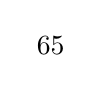
\begin{tikzpicture}
 \Tree [.65  ]
 \end{tikzpicture}
\end{center}
\end{frame}


\begin{frame}{fragile}
\frametitle{Test insert function}

\begin{example}
\begin{enumerate}
\item Now insert 40\\
 \# {\bf let myTree = IntTree.insert 40 myTree};;
\end{enumerate}
\end{example}

\tikzset{every tree node/.style={minimum width=2.5em,draw,circle},
         blank/.style={draw=none},
         edge from parent/.style=
         {draw,edge from parent path={(\tikzparentnode) -- (\tikzchildnode)}},
         level distance=1.5cm, sibling distance=1.5cm}
\begin{center}
\begin{tikzpicture}
 \Tree [.65  [.40 ]  \edge[blank]; \node[blank]{};   ]
\end{tikzpicture}
\end{center}

\end{frame}


\begin{frame}{fragile}
\frametitle{Test insert function}

\begin{example}
\begin{enumerate}
\item Now insert 50\\
 \# {\bf let myTree = IntTree.insert 50 myTree};;
\end{enumerate}
\end{example}

\tikzset{every tree node/.style={minimum width=2.5em,draw,circle},
         blank/.style={draw=none},
         edge from parent/.style=
         {draw,edge from parent path={(\tikzparentnode) -- (\tikzchildnode)}},
         level distance=1.5cm, sibling distance=1.5cm}
\begin{center}
\begin{tikzpicture}
 \Tree [.65  [.40  \edge[blank]; \node[blank]{}; [.50 ] ]  \edge[blank]; \node[blank]{};   ]
\end{tikzpicture}
\end{center}

\end{frame}



\begin{frame}{fragile}
\frametitle{Test insert function}

\begin{example}
\begin{enumerate}
\item Now insert 70\\
 \# {\bf let myTree = IntTree.insert 70 myTree};;
\end{enumerate}
\end{example}

\tikzset{every tree node/.style={minimum width=2.5em,draw,circle},
         blank/.style={draw=none},
         edge from parent/.style=
         {draw,edge from parent path={(\tikzparentnode) -- (\tikzchildnode)}},
         level distance=1.5cm, sibling distance=1.5cm}
\begin{center}
\begin{tikzpicture}
 \Tree [.65  [.40  \edge[blank]; \node[blank]{}; [.50 ]  ]  [.70 ] ]
\end{tikzpicture}
\end{center}

\end{frame}




\begin{frame}{fragile}
\frametitle{Test insert function}

\begin{example}
\begin{enumerate}
\item Now insert 30\\
 \# {\bf let myTree = IntTree.insert 30 myTree};;
\end{enumerate}
\end{example}

\tikzset{every tree node/.style={minimum width=2.5em,draw,circle},
         blank/.style={draw=none},
         edge from parent/.style=
         {draw,edge from parent path={(\tikzparentnode) -- (\tikzchildnode)}},
         level distance=1.5cm, sibling distance=1.5cm}
\begin{center}
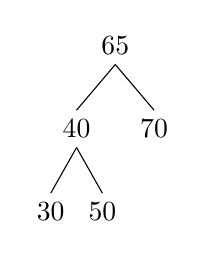
\begin{tikzpicture}
 \Tree [.65  [.40  [.30 ]  [.50 ]  ]  [.70 ] ]
\end{tikzpicture}
\end{center}

\end{frame}


\begin{frame}{fragile}
\frametitle{Test insert function}

\tikzset{every tree node/.style={minimum width=2.5em,draw,circle},
         blank/.style={draw=none},
         edge from parent/.style=
         {draw,edge from parent path={(\tikzparentnode) -- (\tikzchildnode)}},
         level distance=1.5cm, sibling distance=1.5cm}
\begin{center}
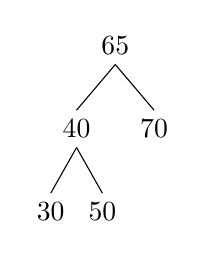
\begin{tikzpicture}
 \Tree [.65  [.40  [.30 ]  [.50 ]  ]  [.70 ] ]
\end{tikzpicture}
\end{center}

\begin{block}{Print myTree using the provided "to\_string" function}
{\bf \# IntTree.to\_string myTree;;}

\vspace*{0.1in}
"Branch (Branch (Branch (Leaf, [30], Leaf), [40], \\~~~~Branch (Leaf, [50], Leaf)), [65], Branch (Leaf, [70], Leaf))"
\end{block}

\end{frame}





\frame[fragile]
\frametitle{Example insert function}


\begin{alertblock}{Example insert function}
\begin{verbatim}
1. let rec insert (x : elt) (t : tree) : tree =
2.  match t with
3.  | Leaf -> Branch (Leaf, [x], Leaf)
4.  | Branch (left, lst, right) -> 
5.     (match Elt.compare x (List.hd lst) with
6.       | Less -> Branch (insert x left, lst, right)
7.       | Greater -> Branch (left, lst, insert x right)
8.       | Equal -> Branch (left, x :: lst, right))
\end{verbatim}
\end{alertblock}
\end{frame}


\frame[fragile]
\frametitle{Example insert function}

\begin{alertblock}{Explanation of the insert function}
\begin{verbatim}
1. let rec insert (x : elt) (t : tree) : tree =
2.  match t with
3.  | Leaf -> Branch (Leaf, [x], Leaf)
4.  | Branch (left, lst, right) -> 
5.     (match Elt.compare x (List.hd lst) with
6.       | Less -> Branch (insert x left, lst, right)
7.       | Greater -> Branch (left, lst, insert x right)
8.       | Equal -> Branch (left, x :: lst, right))
\end{verbatim}
\end{alertblock}

\begin{block}{Explanation}
\begin{description}
\item[\underline{Line \#1}]Insert is a recursive function that takes an element of Elt type and a binary search tree as input arguments and returns the binary tree with the Elt inserted at the correct position
\end{description}
\end{block}

\end{frame}



\frame[fragile]
\frametitle{Example insert function}

\begin{alertblock}{Explanation of the insert function}
\begin{verbatim}
1. let rec insert (x : elt) (t : tree) : tree =
2.  match t with
3.  | Leaf -> Branch (Leaf, [x], Leaf)
4.  | Branch (left, lst, right) -> 
5.     (match Elt.compare x (List.hd lst) with
6.       | Less -> Branch (insert x left, lst, right)
7.       | Greater -> Branch (left, lst, insert x right)
8.       | Equal -> Branch (left, x :: lst, right))
\end{verbatim}
\end{alertblock}

\begin{block}{Explanation}
\begin{description}
\item[\underline{Line \#3}]If t is a Leaf, just insert x at the Leaf and exit
\item[\underline{Line \#5}]If t is a branch, compare x with the first element of the node (remember - it is a list)
\end{description}
\end{block}

\end{frame}




\frame[fragile]
\frametitle{Example insert function}

\begin{alertblock}{Explanation of the insert function}
\begin{verbatim}
1. let rec insert (x : elt) (t : tree) : tree =
2.  match t with
3.  | Leaf -> Branch (Leaf, [x], Leaf)
4.  | Branch (left, lst, right) -> 
5.     (match Elt.compare x (List.hd lst) with
6.       | Less -> Branch (insert x left, lst, right)
7.       | Greater -> Branch (left, lst, insert x right)
8.       | Equal -> Branch (left, x :: lst, right))
\end{verbatim}
\end{alertblock}

\begin{block}{Explanation}
\begin{description}
\item[\underline{Line \#6}]If $x < hd$ then insert it on the left branch of this node 
\item[\underline{Line \#7}]If $x > hd$  then insert it on the right branch of this node
\item[\underline{Line \#8}]If $x = hd$, then add it to the list at this node
\end{description}
\end{block}

\end{frame}



\end{document}
















\begin{frame}{fragile}
\frametitle{Test insert function}

\begin{example}
\begin{enumerate}
\item First create an empty binary tree called myTree \\
        \# {\bf  let myTree = IntTree.empty;;}
\item Insert 65\\
 \# {\bf let myTree = IntTree.insert 65 myTree};;
\end{enumerate}


\end{example}

\tikzset{every tree node/.style={minimum width=2.5em,draw,circle},
         blank/.style={draw=none},
         edge from parent/.style=
         {draw,edge from parent path={(\tikzparentnode) -- (\tikzchildnode)}},
         level distance=1.5cm, sibling distance=1.5cm}
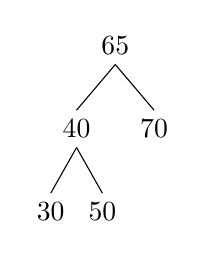
\begin{tikzpicture}
 \Tree [.65  [.40 [.30 ] [.50 ] ]  [.70 ] ]
 \end{tikzpicture}

\end{frame}




\begin{frame}{fragile}
\frametitle{Step 2: Complete insert in {\tt orderedcoll.ml}}
\tikzset{every tree node/.style={minimum width=2em,draw,circle},
         blank/.style={draw=none},
         edge from parent/.style=
         {draw,edge from parent path={(\tikzparentnode) -- (\tikzchildnode)}},
         level distance=1.5cm}
\begin{tikzpicture}
\Tree
[.95     
    [.b ]
    [.c 
    \edge[blank]; \node[blank]{};
    \edge[]; [.d
             \edge[]; {e}
             \edge[blank]; \node[blank]{};
         ]
    ]
]
\end{tikzpicture}

\end{frame}

